\documentclass[9pt,conference]{IEEEtran}
\IEEEoverridecommandlockouts

\usepackage[T2A,T1]{fontenc}
\usepackage[utf8]{inputenc}
\usepackage[english,russian]{babel}
\usepackage{hyperref}
\usepackage{import}

\usepackage{cite}
\usepackage{amsmath,amssymb,amsfonts}
\usepackage{algorithmic}
\usepackage{graphicx}
\usepackage{textcomp}
\usepackage{xcolor}
\def\BibTeX{{\rm B\kern-.05em{\sc i\kern-.025em b}\kern-.08em
    T\kern-.1667em\lower.7ex\hbox{E}\kern-.125emX}}

% translate keywords from english to russian
\def\IEEEkeywordsname{Ключевые понятия}

% redefine modern cyrillic fonts
\renewcommand{\sfdefault}{cmss}
\renewcommand{\rmdefault}{cmr}
\renewcommand{\ttdefault}{cmt}

\begin{document}

\title{Анализ данных с сайта КиноПоиск}

\author{\IEEEauthorblockN{Дмитрий Курносов\IEEEauthorrefmark{1}, Никита Лансков\IEEEauthorrefmark{2}, Михаил Нахатович\IEEEauthorrefmark{3}$^{[0000-0002-6279-1130]}$ и Максим Смольский\IEEEauthorrefmark{4}}
\IEEEauthorblockA{
	Высшая школа прикладной математики и вычислительной физики\\
	Санкт-Петербургский политехнический университет\\
    Санкт-Петербург, Россия \\
    Email: \IEEEauthorrefmark{1}dima2202888@yandex.ru, \IEEEauthorrefmark{2}nl516@yandex.ru, \IEEEauthorrefmark{3}mish\_1998@mail.ru, \IEEEauthorrefmark{4}mithridatus@mail.ru
    }
}

\maketitle

\begin{abstract}
В статье описывается процесс анализа данных с сайта КиноПоиск. В рамках статьи рассмотрены процессы получения и хранения данных, а также их последующей обработки для решения поставленных задач: поиск взаимосвязи между различными характеристиками фильмов, построение распределений фильмов по различным критериям.
\end{abstract}

\begin{IEEEkeywords}
Большие данные, распределённые вычисления
\end{IEEEkeywords}

\section{Введение}

Индустрия фильмов развивается с каждым годом и является важной частью в жизни каждого человека. Также растёт интерес к кинопрокату, ежегодно растёт оборот денежных средств в киноиндустрии, а также качество съёмки и число людей, задействованных в процессе работы над новыми фильмами.

КиноПоиск - крупнейший русскоязычный интернет-сервис о кино. Данный сервис предоставляет информацию о различных фильмах, актёрах, новостях кино и т.д.

В данной работе представлен анализ данных о фильмах: рассмотрены взаимосвязи между 
различными характеристиками фильмов и построены распределения фильмов по различным критериям. В рамках данной работы мы делали упор на статистические методы анализа данных.

\section{Данные}

\subsection{Получение данных}

Для скачивания данных использовался сторонний API для доступа к актуальной информации КиноПоиска. Так как данный API предоставляет информацию о фильме только по его идентификатору, для получения всех идентификаторов фильмов был выполнен парсинг самого сайта КиноПоиск. Коннектор написан на языке Python с использованием пакета PyMongo для работы с MongoDB из Python. Всего было выкачено 654165 фильмов. Объём данных составил 3.4 Гб.

\subsection{Структура данных}

Выгруженную информацию о фильмах можно поделить на блоки, представленные на Рис.~\ref{fig:1}. Каждый фильм содержит некоторые общие сведения такие как название, год производства, жанры и т.д. Также есть список создателей, то есть список всех актёров, режиссёров и т.д., задействованных в создании фильма. Различные рейтинги, в число которых входит рейтинг из базы IMDb. Рецензии зрителей и бюджет фильма, в который также входят сборы.

\begin{figure}[ht!]
	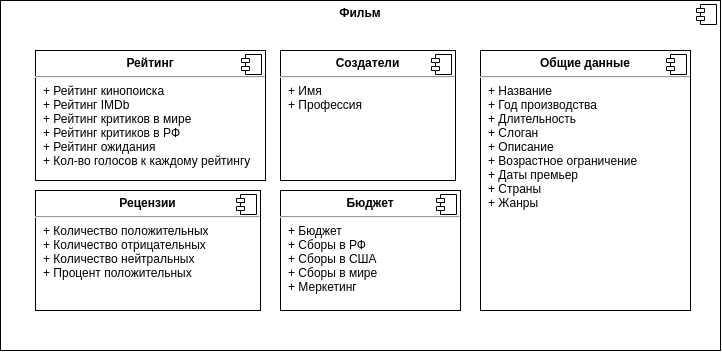
\includegraphics[width=\linewidth]{../report/images/dataStructure}
	\caption{Схема представления данных.}
	\label{fig:1}
\end{figure}



\section{Статистические задачи}
\subsection{Корреляция оценок зрителей и критиков}

\import{tasks/}{rank_correlation.tex}

\subsection{Корреляция рейтинга КиноПоиска и рейтинга IMDb}

\import{tasks/}{rating_rank_correlation.tex}

\subsection{Распределение фильмов по странам}

\import{tasks/}{count_films_by_countries_task.tex}

\subsection{Распределение фильмов по прибыльности}

\import{tasks/}{films_by_budget.tex}

\subsection{Распределение фильмов между странами по годам}

\import{tasks/}{films_by_countries_year.tex}

\subsection{Распределение фильмов по возрастным ограничениям и годам}

\import{tasks/}{films_number_by_age_limit_calculation.tex}

\subsection{Средний рейтинг российских фильмов по годам}

\import{tasks/}{russia_rating_by_year.tex}

\section{Исследовательские задачи}
\subsection{Прогноз количества фильмов по жанрам на 10 лет}

\import{tasks/}{films_number_by_genre_prediction.tex}

\section{Дальнейшие исследования}

Во-первых, мы хотим построить модель, с помощью которой можно предсказывать рейтинг фильма по его создателям, например, актёрам, режиссёрам и сценаристам, а также другим данным, таким как жанры или страны производители. Для этой задачи нужно понять, как эффективно связать категориальные признаки с итоговым числовым значением. Во-вторых, мы хотим выкачать сериалы и выполнить статистические задачи для них.

\begin{thebibliography}{00}
\bibitem{b1} Сайт «КиноПоиск». [Электронный ресурс]. Режим доступа: \url{https://www.kinopoisk.ru/}
\bibitem{b2} Сайт «MongoDB». [Электронный ресурс]. Режим доступа: \url{https://www.mongodb.com/}

\end{thebibliography}

\end{document}
